

% DICHIARAZIONE myFOOTNOTES
\newcommand{\citPORVA}{\nota{PORVA: Inertial Measurement Unit}{}}

%%%%% Capitolo 1 %%%%%

\label{02-chapter}
%\usepackage{wrapfig}
\begin{wrapfigure}{l}{90mm}
  \begin{center}
    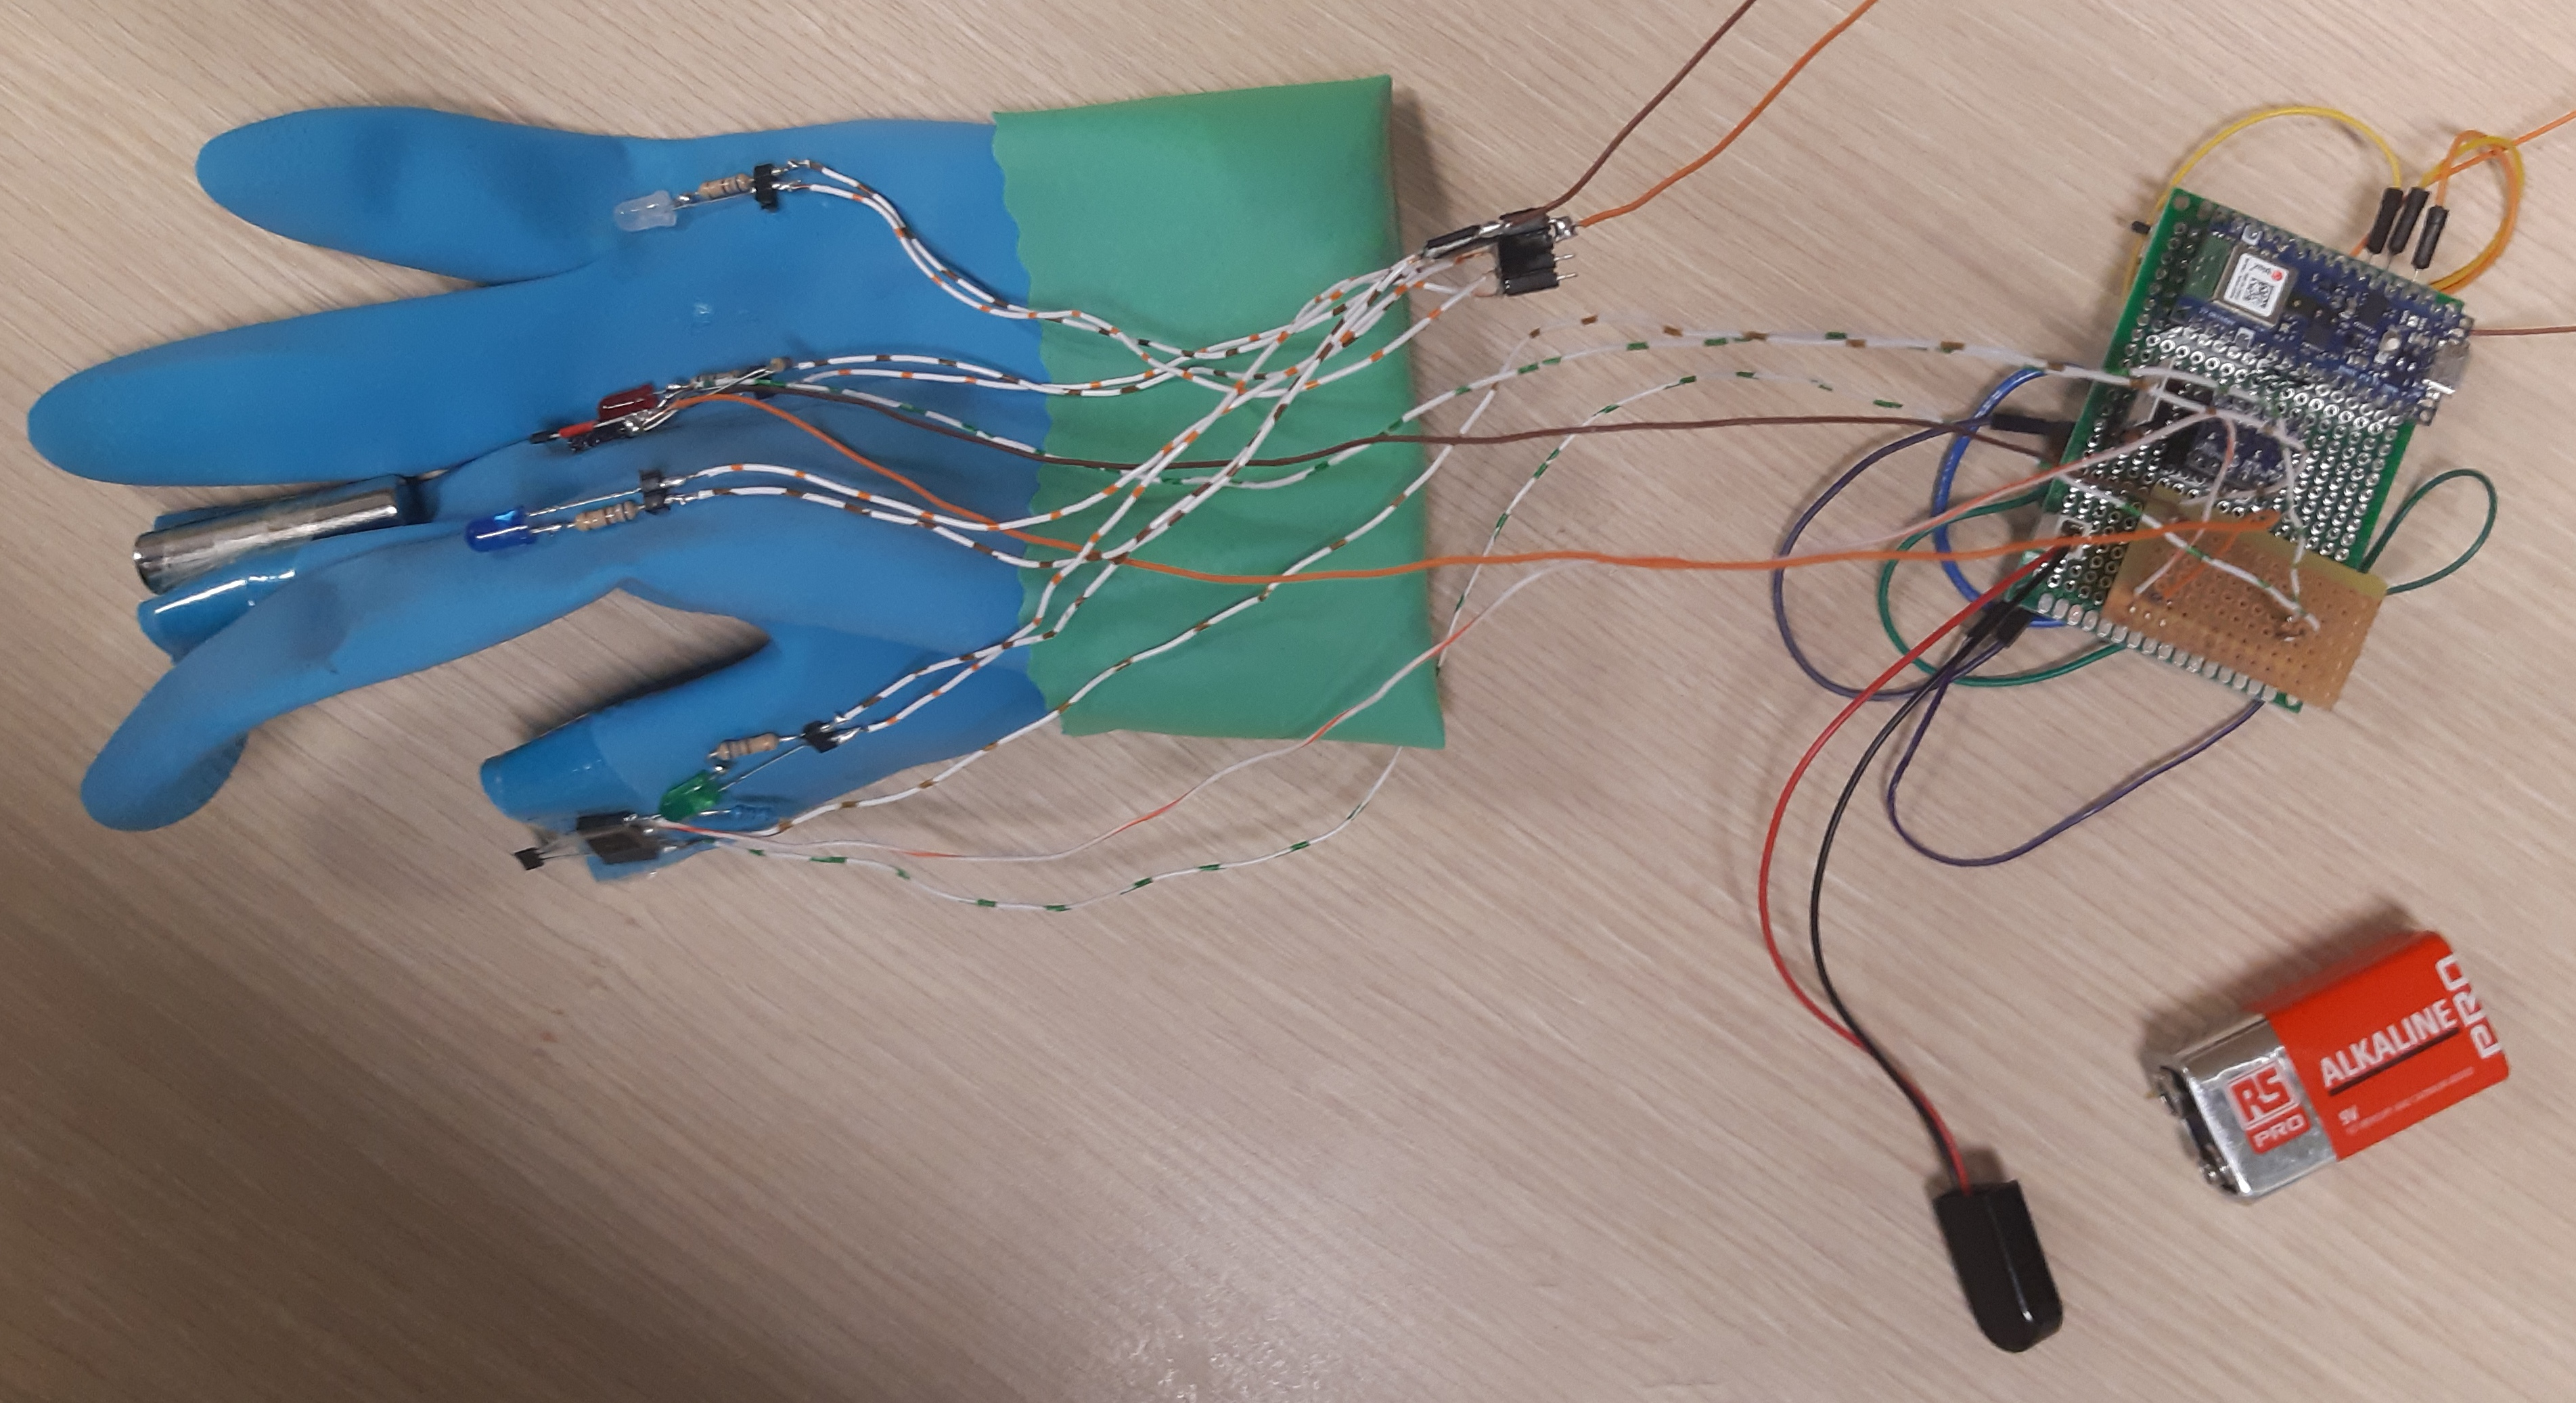
\includegraphics[width=0.48\textwidth]{figures/Guanto_Finale (1).jpg}
  \end{center}
    \caption{Immagine Finale del Guanto per il Riconoscimento di uno Schiocco di Dita}
%\end{wrapfigure}
\end{wrapfigure}

Utilizzando due sensori di Hall, posizionati su un guanto di gomma, uno sul retro del pollice e l'altro sulla nocca del dito medio, una calamita attaccata al retro del medio, e l'Arduino Nano 33 BLE Sense sul quale è caricato lo sketch con il modello di machine learning, sono stato in grado di rivelare quando vengono fatte schioccare le dita,\comment{e se la rete neurale ha una confidenza che reputo sufficiente} e quando accade \comment{attivo}4 led incollati sul guanto si accendono.\\

Il flusso di lavoro\comment{workflow} che ho adottato è il seguente:
\par

\begin{itemize}
    \item {Raccolta dei dati dai sensori tramite sketch Arduino, che dovranno poi essere scritti sulla porta seriale, sempre dallo stesso sketch.}
    \item {Collezione dei dati scritti sul seriale, e salvataggio degli stessi su fogli con estensione ".csv", tramite script python.}
    \item {Inoltro dei file ".csv" appena creati sulla piattaforma Edge Impulse, con seguente creazione ed allenamento della rete neurale, che verrà poi inserita in una libreria Arduino per il dislocamento sulla scheda Nano.}
    \item {Infine, creazione di un nuovo sketch Arduino per l'utilizzo della libreria fornita da Edge.}\\
\end{itemize}

\newpage{}



\section{Raccolta Dati tramite Sketch Arduino} \label{sezione 2-1}
Per prima cosa ho creato un semplice prototipo su breadboard in cui ho collegato una scheda Arduino UNO come mostrato in \riferimento{IMAGE - GDA ARDUINO UNO}{Figura 2.2}.
Ho usato questa scheda in una prima prova, per la possibilità dell'Arduino UNO di inviare e ricevere segnali a 5 V, visto che i sensori devono essere alimentati a 5 V, ed i valori in uscita dal sensore hanno range tra\\ 0 V - 5 V, valori che normalmente \textbf{non} possono essere accettati, come scritto in precedenza, dall'Arduino Nano.
Questo problema è facilmente risolvibile con convertitori di tensione generici per \\5 V$\rightarrow{}$3.3 V, convertitori che sono stati infatti adottati in seguito.\\

\label{IMAGE - GDA ARDUINO UNO}
\begin{figure}[H]
    \centering
    \caption{Esempio di hardware per la lettura dei sensori Hall}
    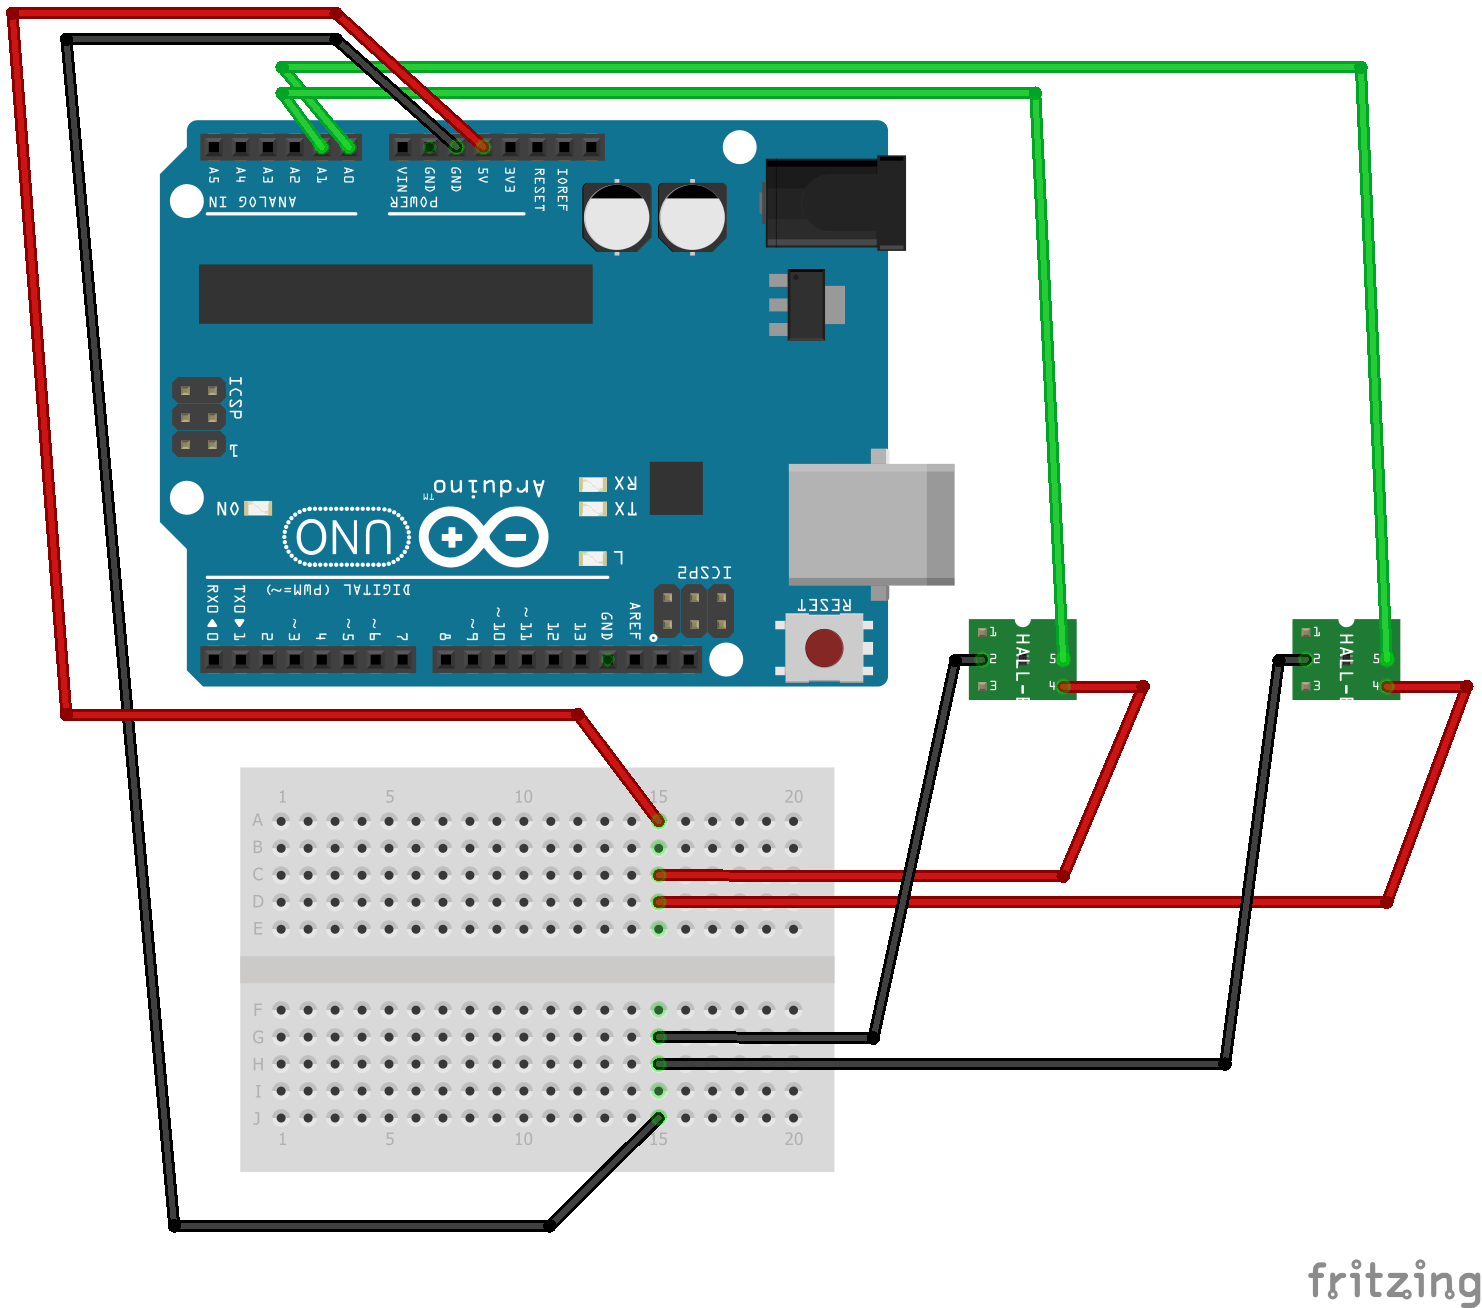
\includegraphics[width=\textwidth]{figures/Fritzing - GDA_from_Hall_Sensors_I.png}
\end{figure}

\newpage{}

Una volta visto come raccogliere dati, e scelto un magnete tra quelli disponibili in laboratorio, che dia una variazione consistente se mosso vicino ai sensori, ho portato il progetto sull'Arduino Nano, tramite vari shifter di tensione, come accenato prima, ed alimentando il tutto a batteria (9 V). Lo schema del progetto è mostrato nella \riferimento{IMAGE - GDA ARDUINO NANO}{Figura 2.3}:
\label{IMAGE - GDA ARDUINO NANO}
\begin{figure}[H]
    \centering
    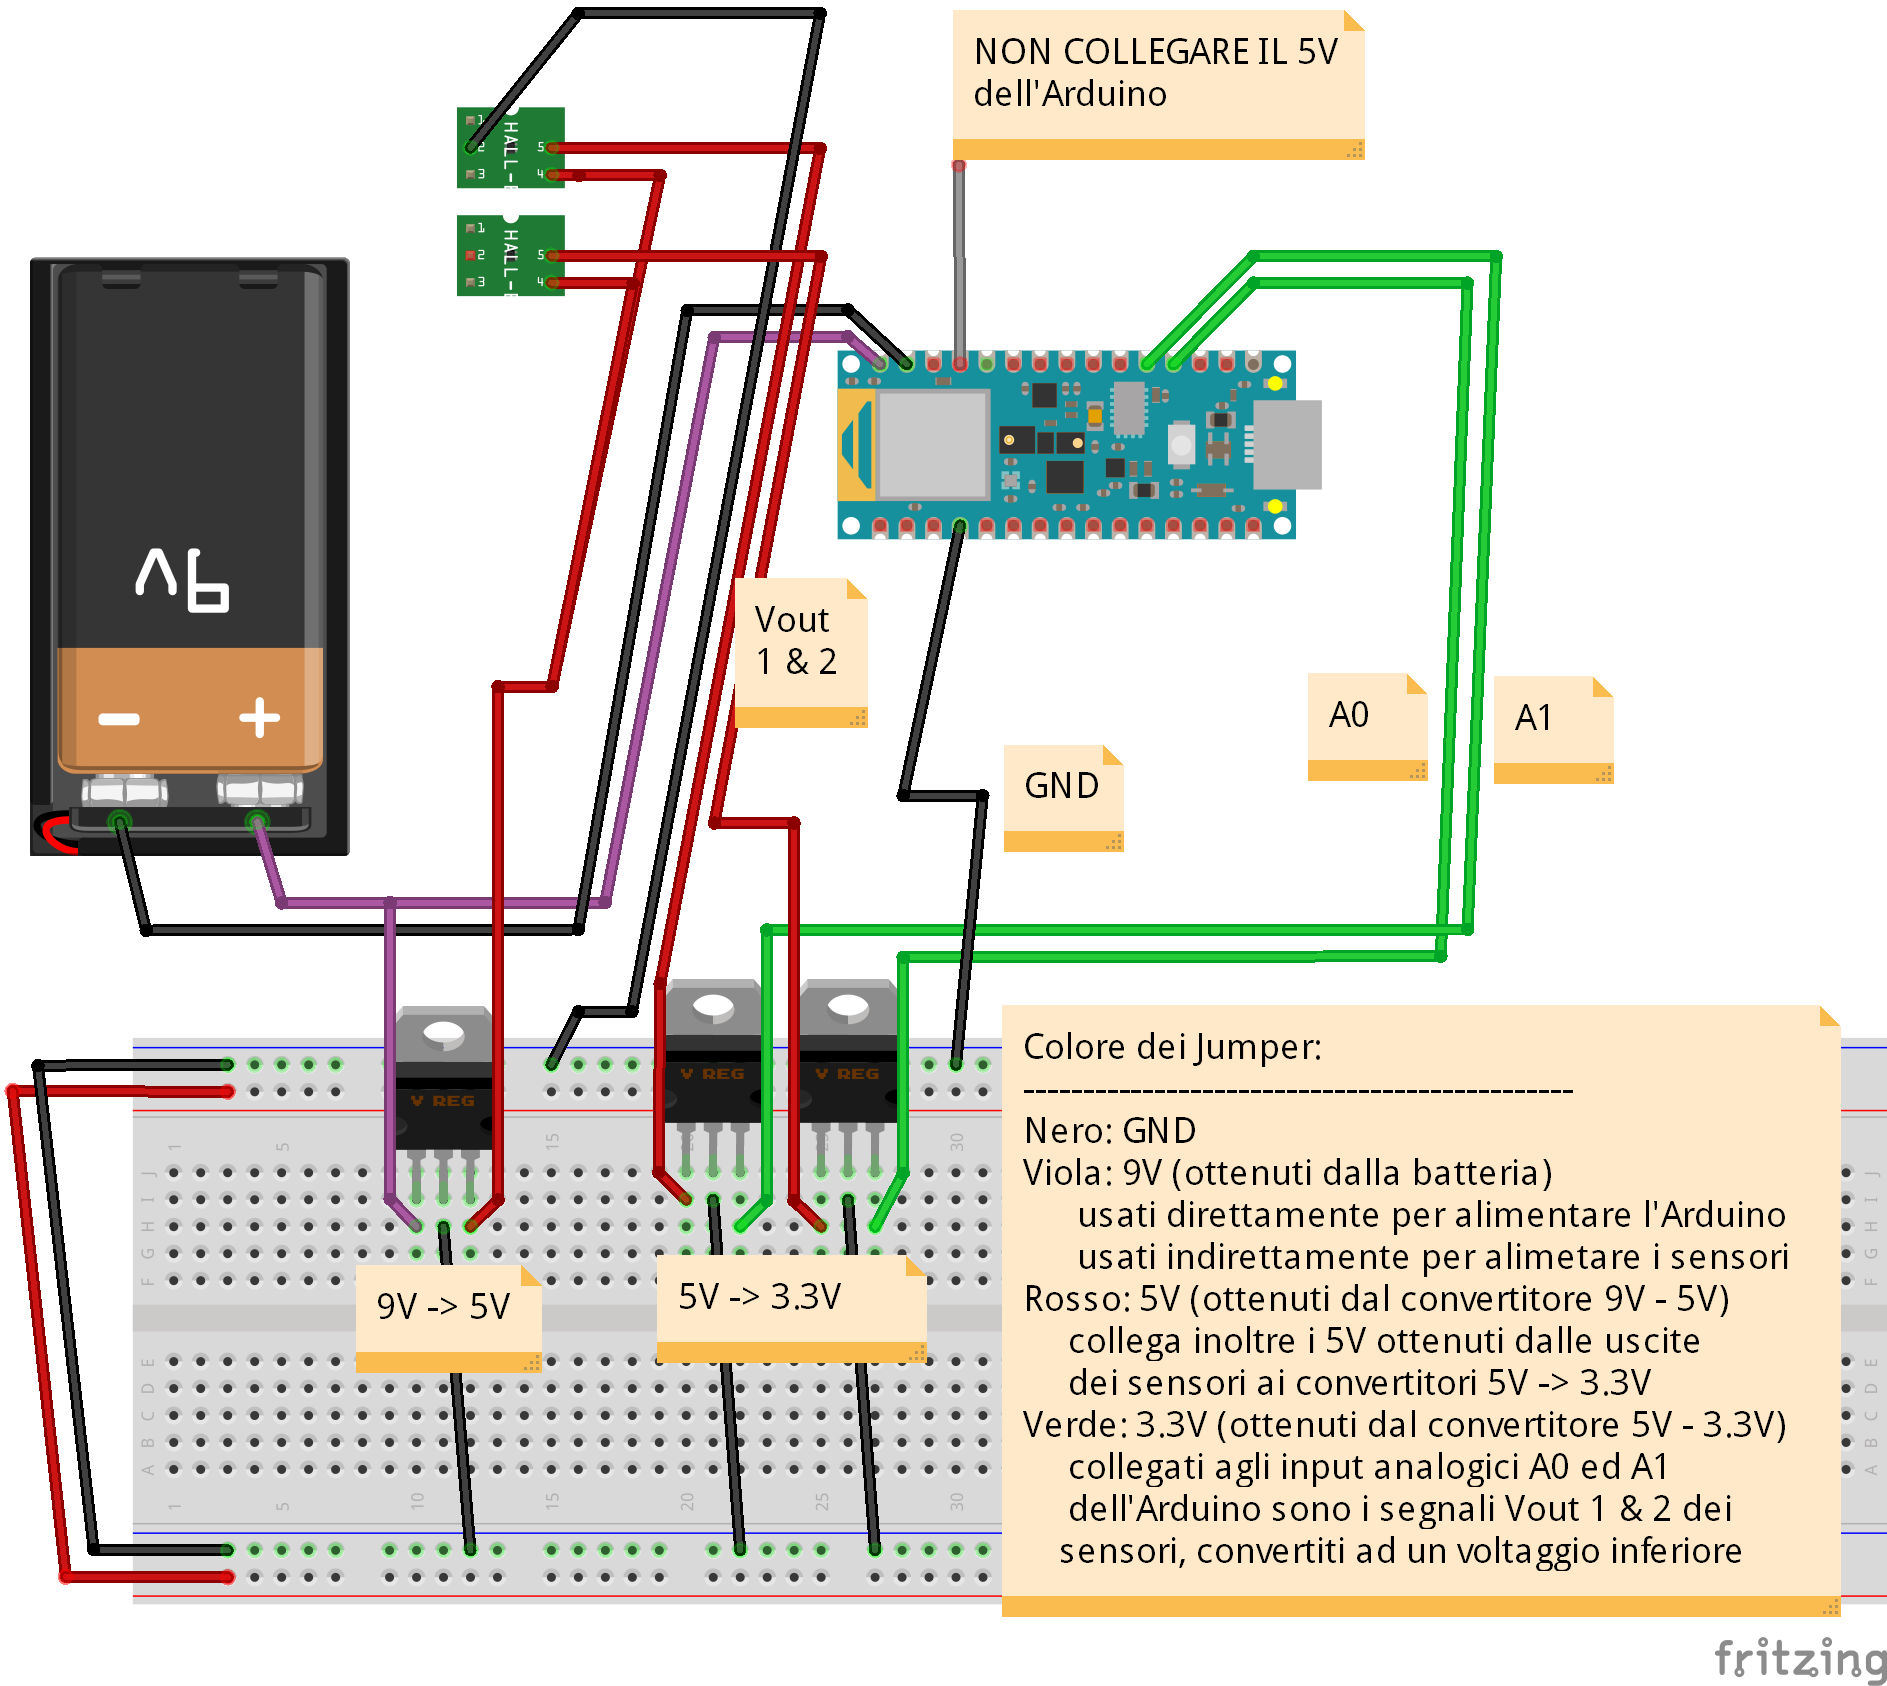
\includegraphics[width=\textwidth]{figures/2.1. Second Configuration -with more Names_bb.png}
    \caption{Esempio di hardware per la lettura dei sensori Hall su scheda Arduino Nano 33 BLE Sense}
\end{figure}

Tramite questa configurazione è possibile collegare l'Arduino Nano al PC per la raccolta dati tramite scrittura su seriale, utilizzando nel codice principalmente due funzioni: "AnalogRead(...)" e "Serial.print(...)", di seguito la parte principale del codice utilizzato per la lettura dai sensori:

\newpage{}

\begin{lstlisting}[language=Arduino]
void loop(){ // Lettura di due sensori
    String value_on_pollice = String(AnalogRead(A0));
    String value_on_medio = String(AnalogRead(A1));
    String timestamp = String(millis());
    Serial.println(timestamp + "," + value_on_pollice + "," + value_on_medio)
}
\end{lstlisting}






\subsection{Protocollo Edge Impulse} \label{sezione 2-1-1}
Il formato per la scrittura dei dati sul seriale:
\begin{lstlisting}[language=Arduino]
timestamp + "," + value_on_pollice + "," + value_on_medio
\end{lstlisting}
Non è stato scelto a caso, di fatti il servizio Edge Impulse richiede che i fogli ".csv" abbiano il seguente protocollo o formato, per la successiva lettura dei dati:
\begin{lstlisting}[language=HTML]
timestamp, name_value_1, name_value_2, name_value_3, name_value_4
0, 23.34, 2131.23, 321.23, 232.4
12, 23.34, 2131.23, 321.23, 232.4
23, 22.36, 2003.10, 321.23, 567.8
45, 26.24, 2056.40, 321.23, 567.9
54, 25.38, 1233.23, 321.23, 567.4
...
\end{lstlisting}
Questo formato sarà poi creato per intero dallo script python di cui parlerò nella prossima sezione, in ogni caso, è necessario che i fogli ".csv" abbiano tutti come prima colonna il "timestamp", così che Edge Impulse possa dare ad ogni dato fornitogli un marchio temporale, ecco il perché dell'omonima variabile durante la scrittura sul seriale (scritta appunto per prima).\\
Successivamente il sito si aspetta tutti i dati raccolti dai vari sensori, che vengono appunto scritti sul seriale, dopo il timestamp.

\subsection{Primo Prototipo del Guanto per la Raccolta Dati} \label{sezione 2-1-2}
A questo punto è necessario creare un prototipo per la raccolta dati, in quanto ho necessità di registrare i vari dati durante il movimento prestabilito, uno schiocco di dita.
Il prototipo con i sensori letteralmente incollati sopra è fondamentale per questo passaggio in quanto ho bisogno di avere i sensori nella stessa posizione, sia per l'allenamento, che per il test della rete neurale, se i sensori si muovessero ogni volta, addestrerei la rete su valori "traslati" rispetto alla fase di test, questo porterebbe sicuramente ad errori, non facilmente risolvibili.\par
Di seguito alcune foto su come ho incollato calamita e sensori, che poi collegherò alla scheda Nano come visto in precedenza in \riferimento{IMAGE - GDA ARDUINO NANO}{Figura 2.2}.

\label{IMAGE - GUANTO}
\begin{figure}[H]
    \centering
    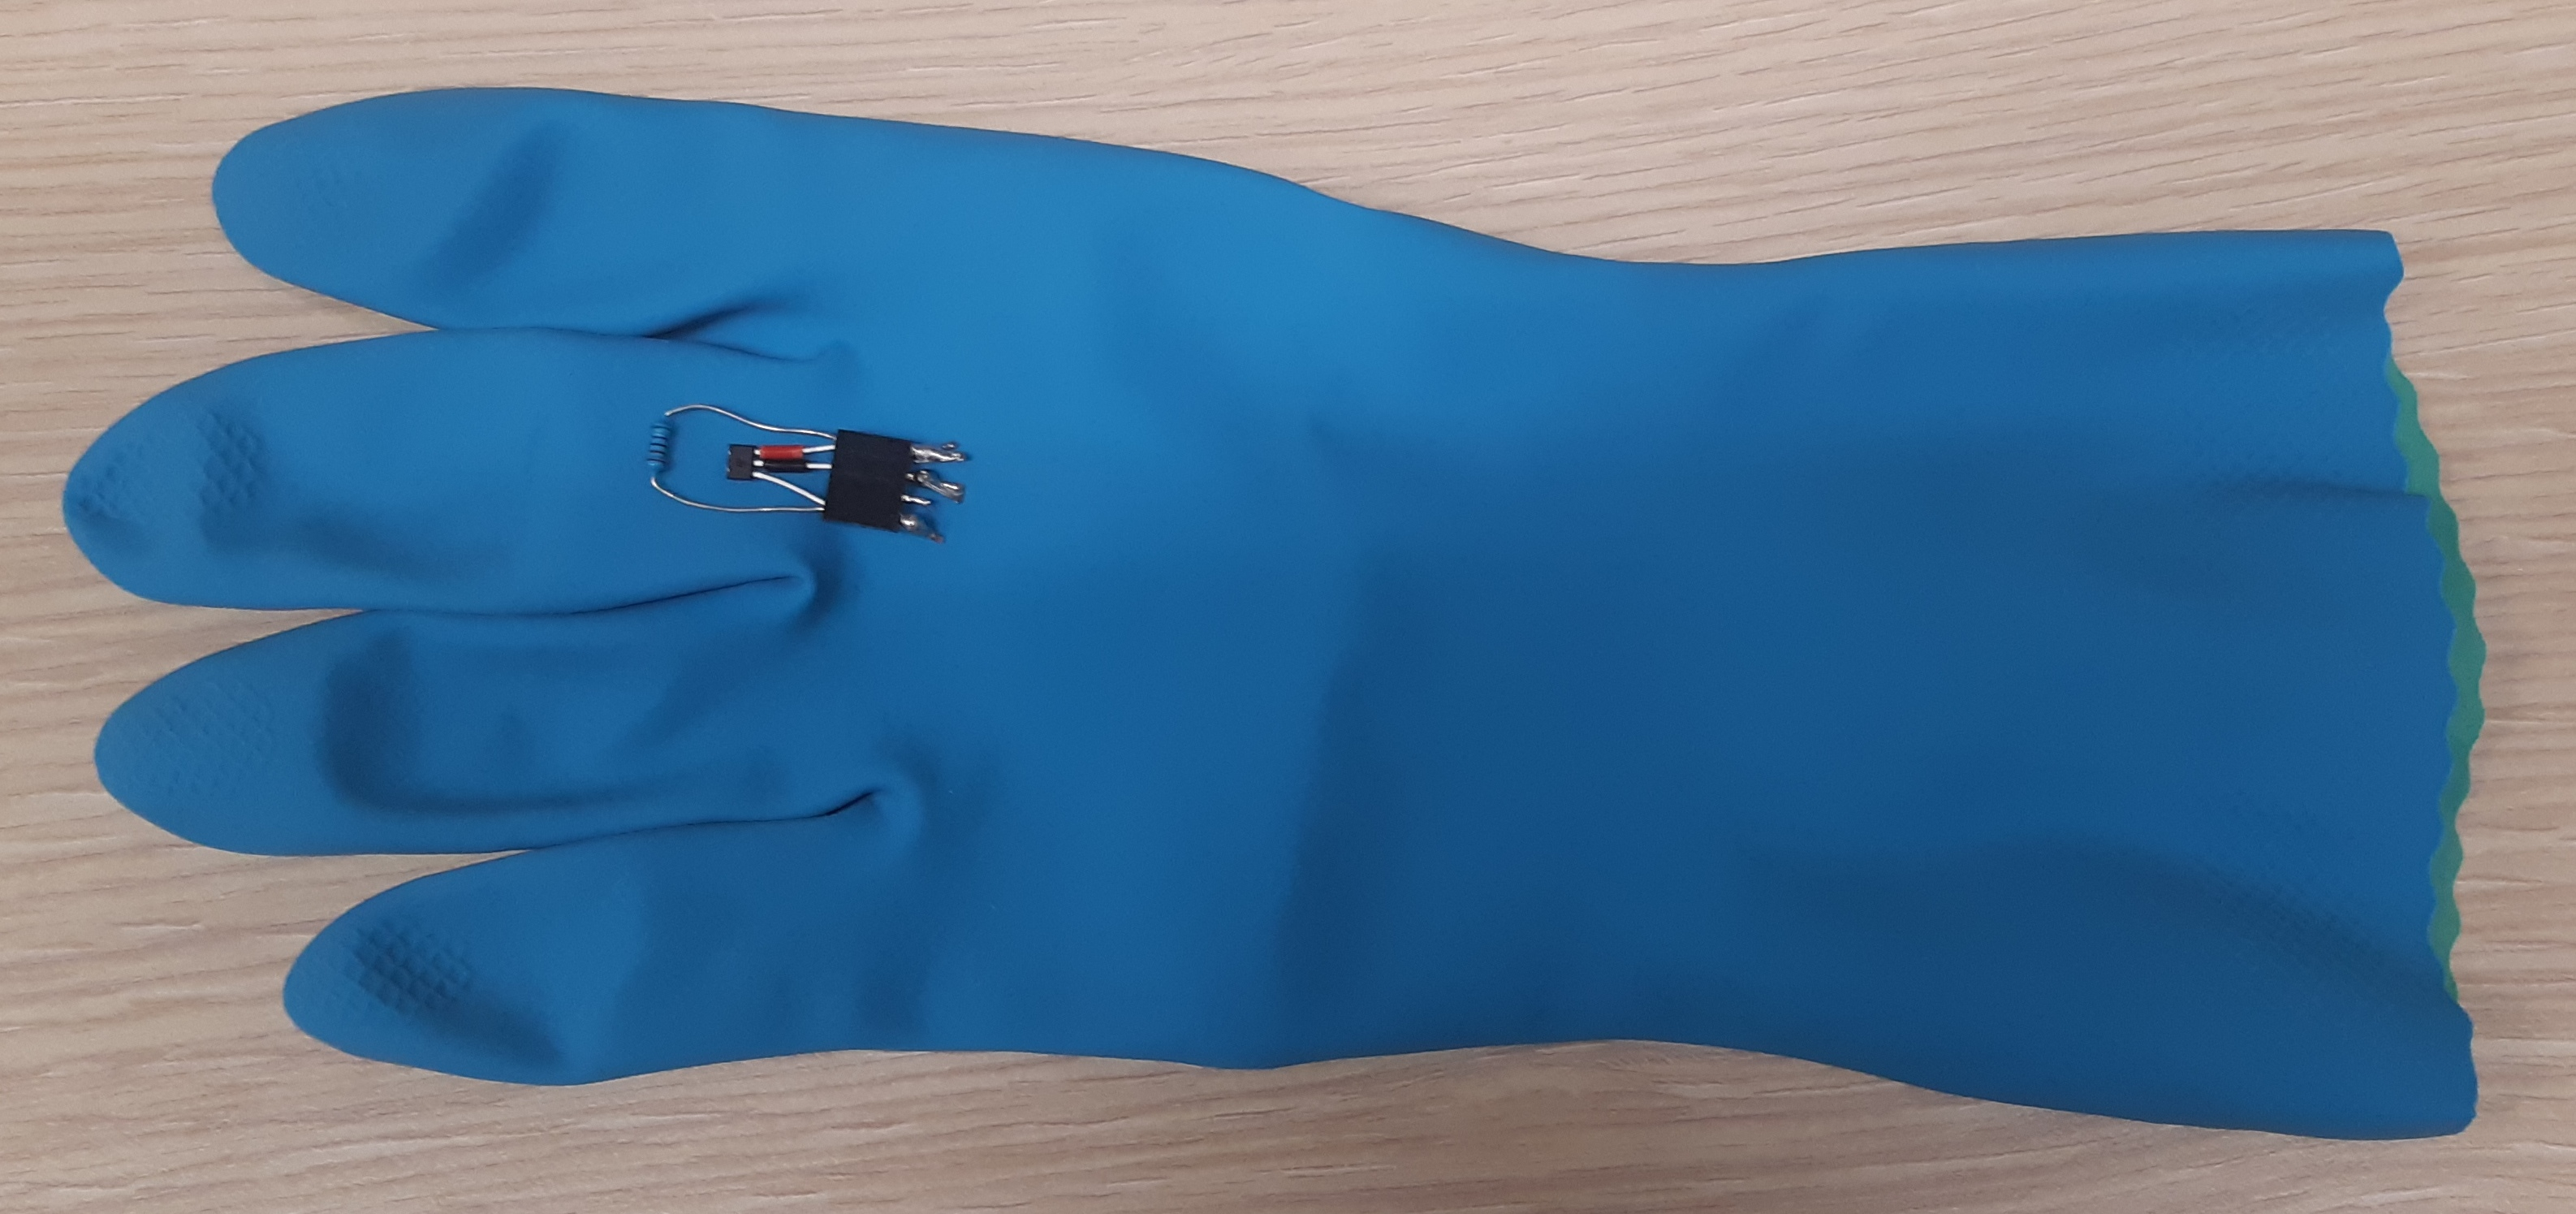
\includegraphics[width=115mm]{figures/Guanto_1 (1).jpg}
    \caption{Primo prototipo del guanto (sensore sul medio)}
    
    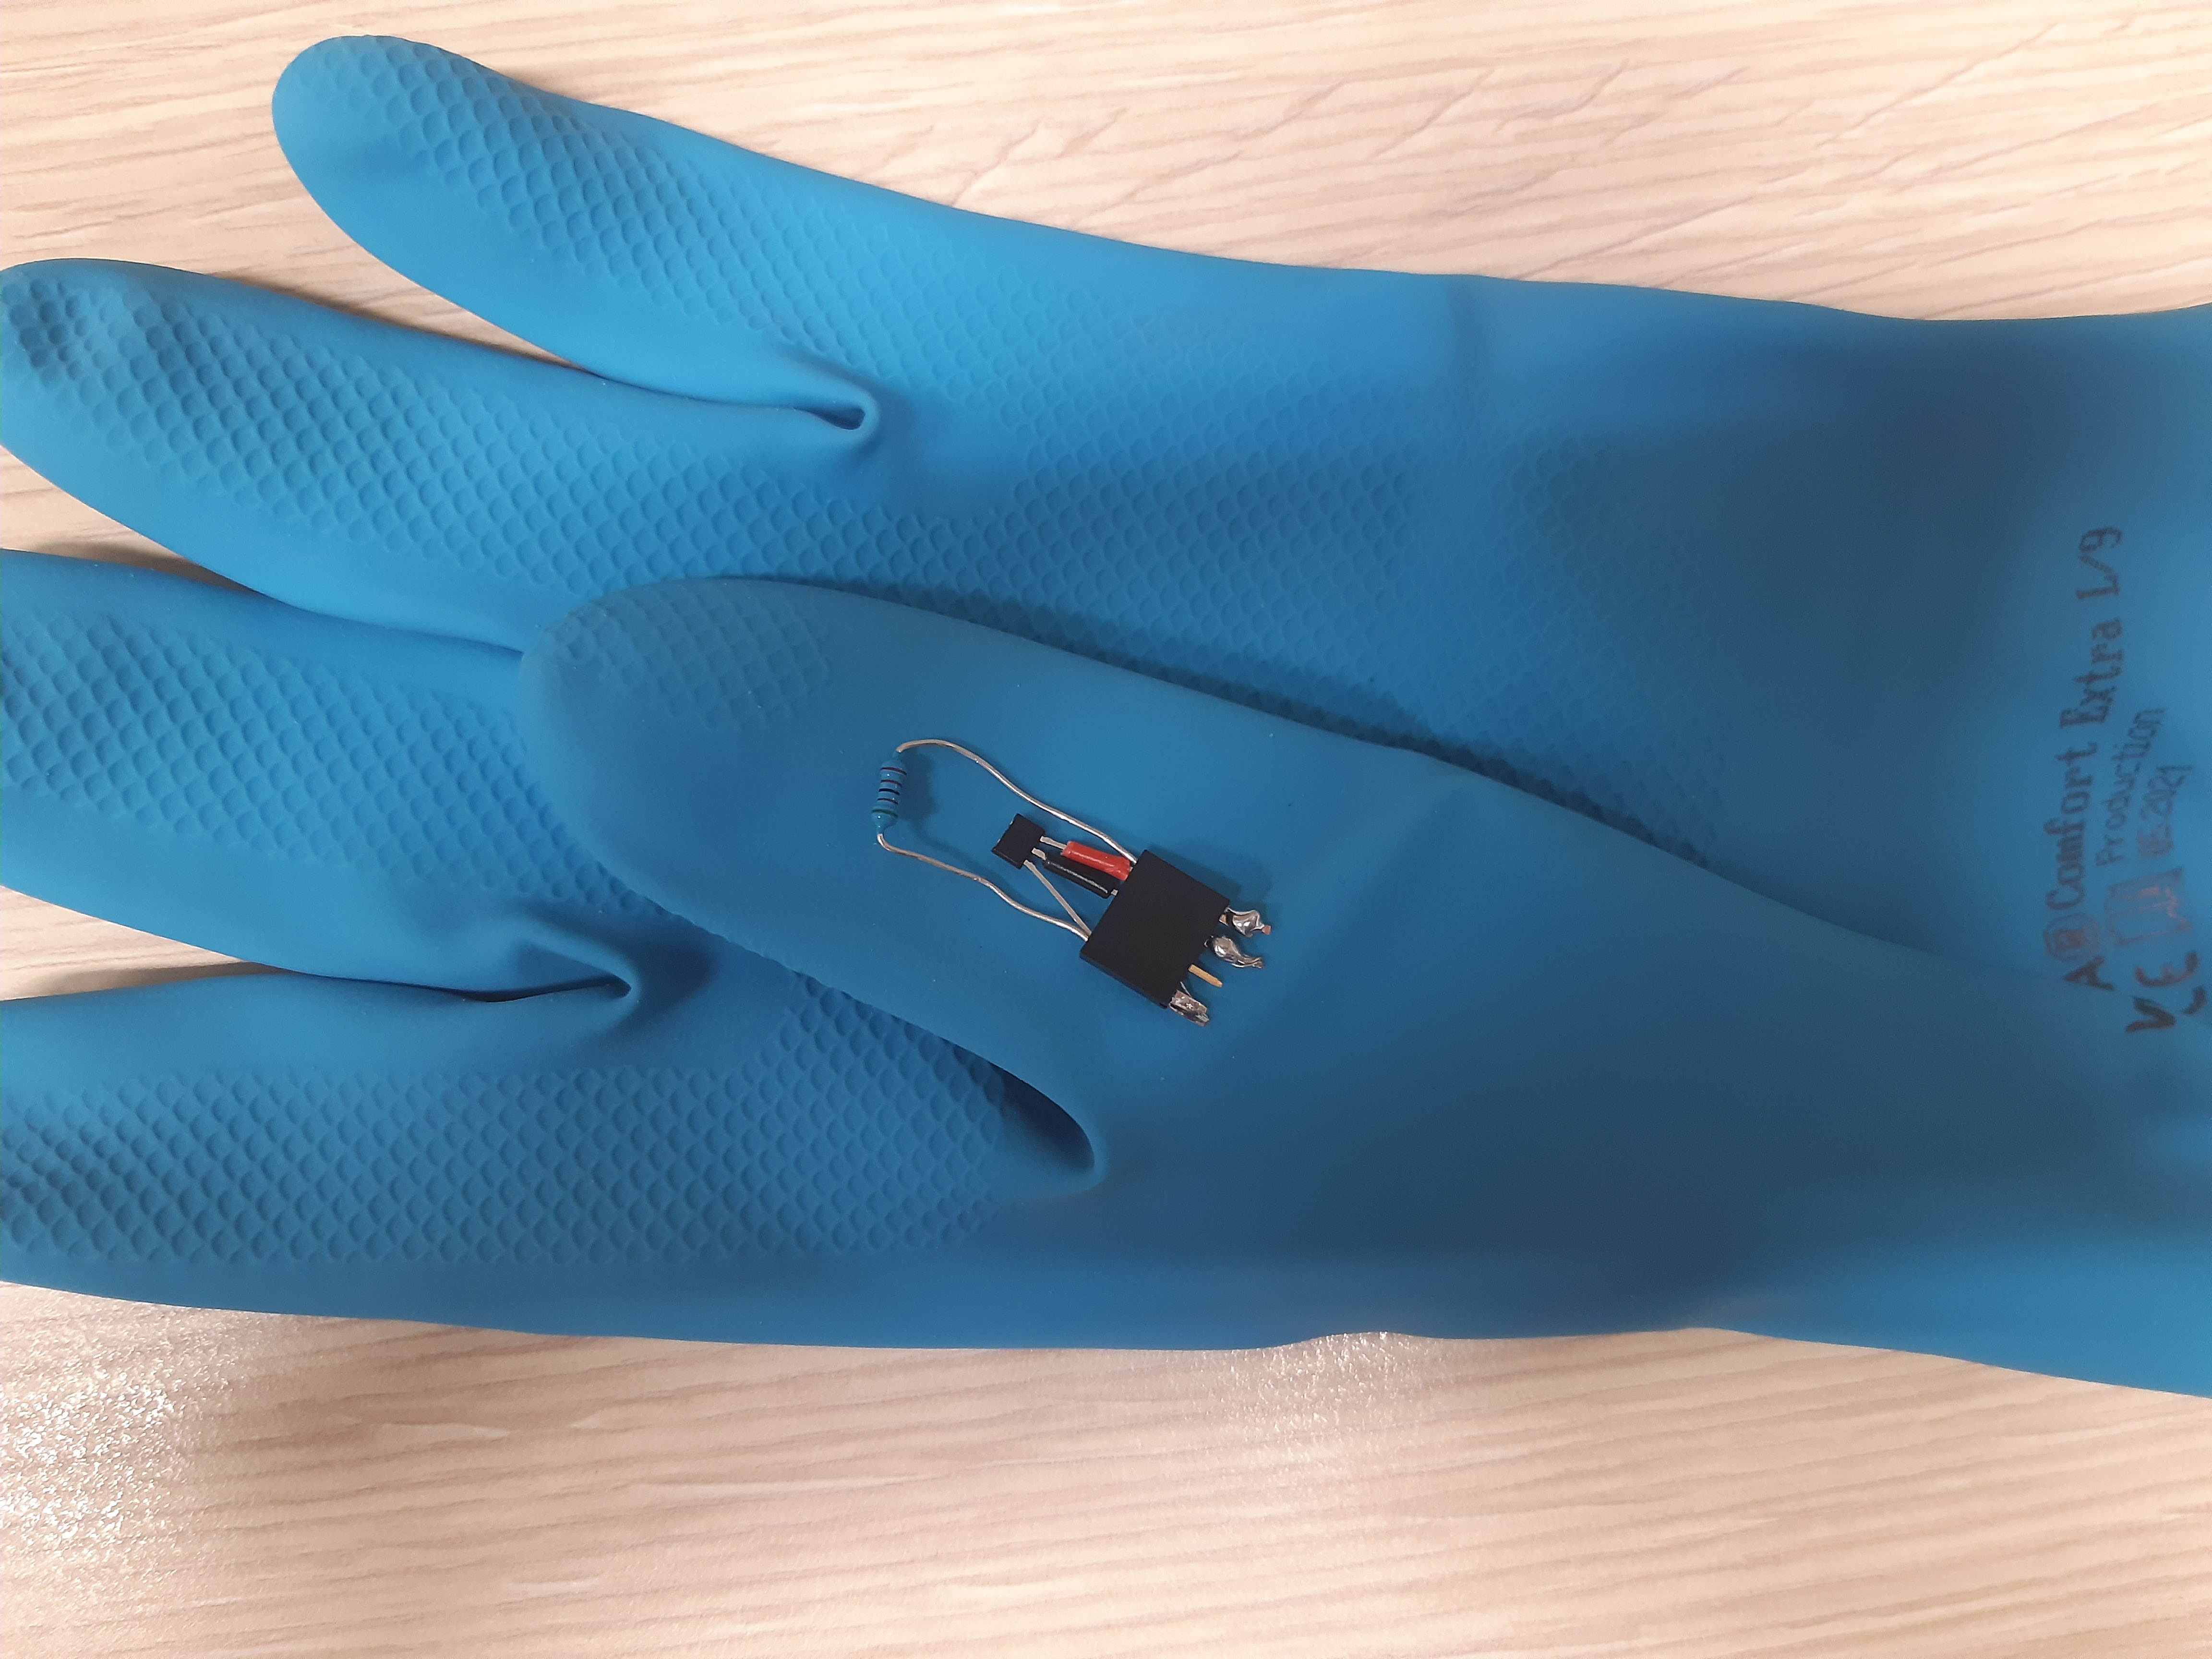
\includegraphics[width=115mm]{figures/Guanto_2.jpg}
    \caption{Sensore sul pollice}
    
    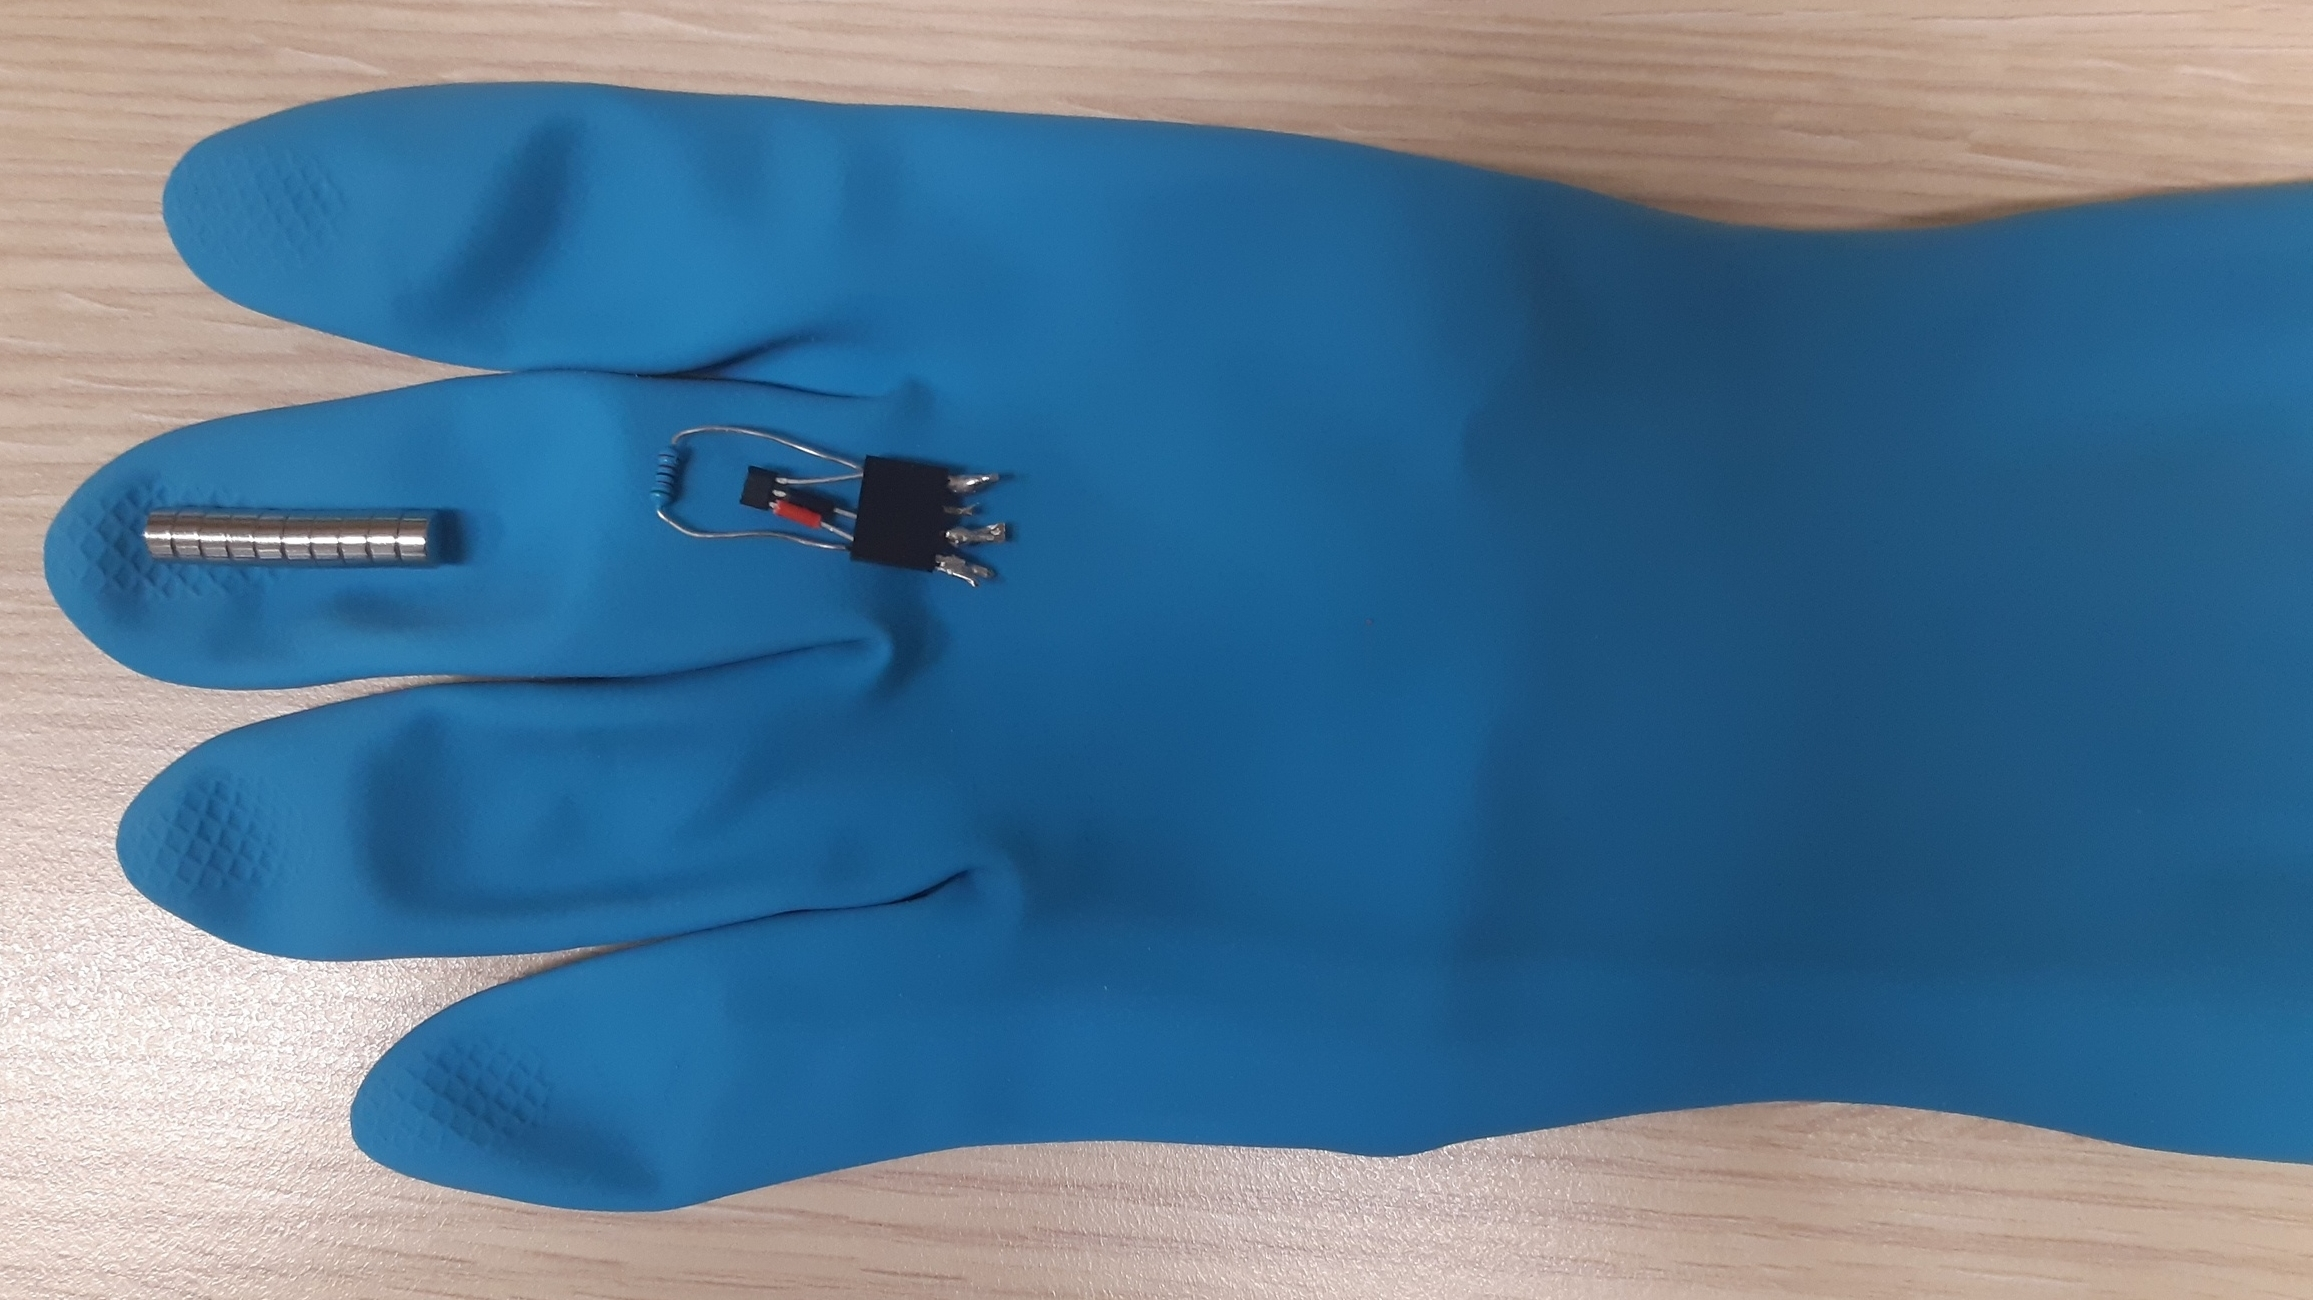
\includegraphics[width=115mm]{figures/guanto_3--3---1-.jpg}
    \caption{Sensore sul medio e calamita}
\end{figure}

\section{Script Python per la Scrittura Automatica di Fogli ".csv"} \label{sezione 2-2}
Ricevendo i dati tramite seriale è possibile utilizzare una libreria python "pyserial" per la lettura di questi; il procedimento è il seguente:
una volta collegata la scheda Arduino ad una porta seriale ad esempio "COM3", possiamo creare uno script python che utilizza la libreria o modulo "pyserial" in questo modo:
\begin{lstlisting}[language=Python]
import serial

MAX_CICLES = 100
EMPTY_DATA_SRING = "b''"
INITIAL_DATA_TO_INGNORE = len("b'")
FINAL_DATA_TO_INGNORE = len("'\n\r")

arduino = serial.Serial(
    port = 'COM3',
    baudrate = 115200, 
    timeout = .1
)

for _ in range(MAX_CICLES):
    data = str(arduino.readline())
    
    if data != EMPTY_DATA_SRING:
        return data[INITIAL_DATA_TO_INGNORE:-FINAL_DATA_TO_INGNORE]
\end{lstlisting}
\myNOTE{Questo breve script premette solo di leggere una singola riga dal serial. \\
Andrà ripetuto più volte per leggere tutti i dati passati dall'Arduino.}
\par{}Una volta ricevuti i dati dall'Arduino, e opzionalmente salvati in una variabile, sarà possibile scriverli su un nuovo foglio ".csv".\\
Decidendo il percorso dove salvare il file, ad esempio\\ "\textit{C:$\backslash{}$Users$\backslash{}$Amministratore$\backslash{}$Cartella\_Files\_CSV$\backslash{}$nuovo\_file.csv}", possiamo creare il file e trascriverci i dati da una variabile utilizzando la funzione python "open(...)":
\begin{lstlisting}[language=Python]
absolute_path = "C:\Users\Amministratore\Cartella_Files_CSV\nuovo_file.csv"
with open(absolute_path, "w") as file:
    file.write(dati_raccolti_dallArduino_tramite_la_precedente_funzione)
\end{lstlisting}

È possibile, ovviamente, ripetere tutto il procedimento quante volte vogliamo, finendo con\comment{pordandoci ad}  avere a disposizione molti fogli ".csv" con all'interno i dati ricavati dai sensori tramite la scheda Arduino, dati che saranno la base dell'addestramento della rete neurale.\\

Per la raccolta dati nel mio specifico caso ho fatto girare lo script python sia durante uno schiocco di dita, ma anche mentre tenevo\comment{ho tenuto} la mano ferma in varie posizioni diverse, ad esempio "mano aperta", "pugno chiuso" ecc., ed infine ho registrato anche alcune "anomalie", ovvero gesti che non devono essere classificati, questo per aiutare la rete neurale a distinguere in futuro tra uno schiocco di dita e tra un qualsiasi altro gesto, dopotutto lo scopo è far accendere dei led \textbf{solo} quando viene rivelato uno schiocco.
\newpage{}
\section{Utilizzo della Piattaforma Edge Impulse} \label{sezione 2-1}
Avendo a mia disposizione\comment{un totale di} più di 10 minuti di dati raccolti\comment{in questi file} nei file ".csv", ho creato ed addestrato la rete neurale utilizzando la piattaforma Edge Impulse:\\
Ho iniziato dopo la registrazione sul sito, creando un nuovo progetto, e caricando tutti i file creati in precedenza sull'apposita pagina, che si può trovare su 'Edge Impulse'$\rightarrow{}$'Data Aquisition'$\rightarrow{}$'Upload existing data', in questa pagina viene richiesto di caricare i file da inviare ad Edge, e scegliere un "label" che rappresenti tutti i file caricati, la label sarà poi utilizzata da Edge come classe di classificazione per la rete neurale.

Dopo viene chiesto di creare un cosiddetto "Impulso", ovvero il \textit{workflow} che implementerà Edge per l'addestramento del modello di machine learning. Per questo progetto la struttura dell'Impulso che ho scelto è la seguente:
\label{IMAGE - IMPULSO COMPLETO}
\begin{figure}[H]
    \centering
    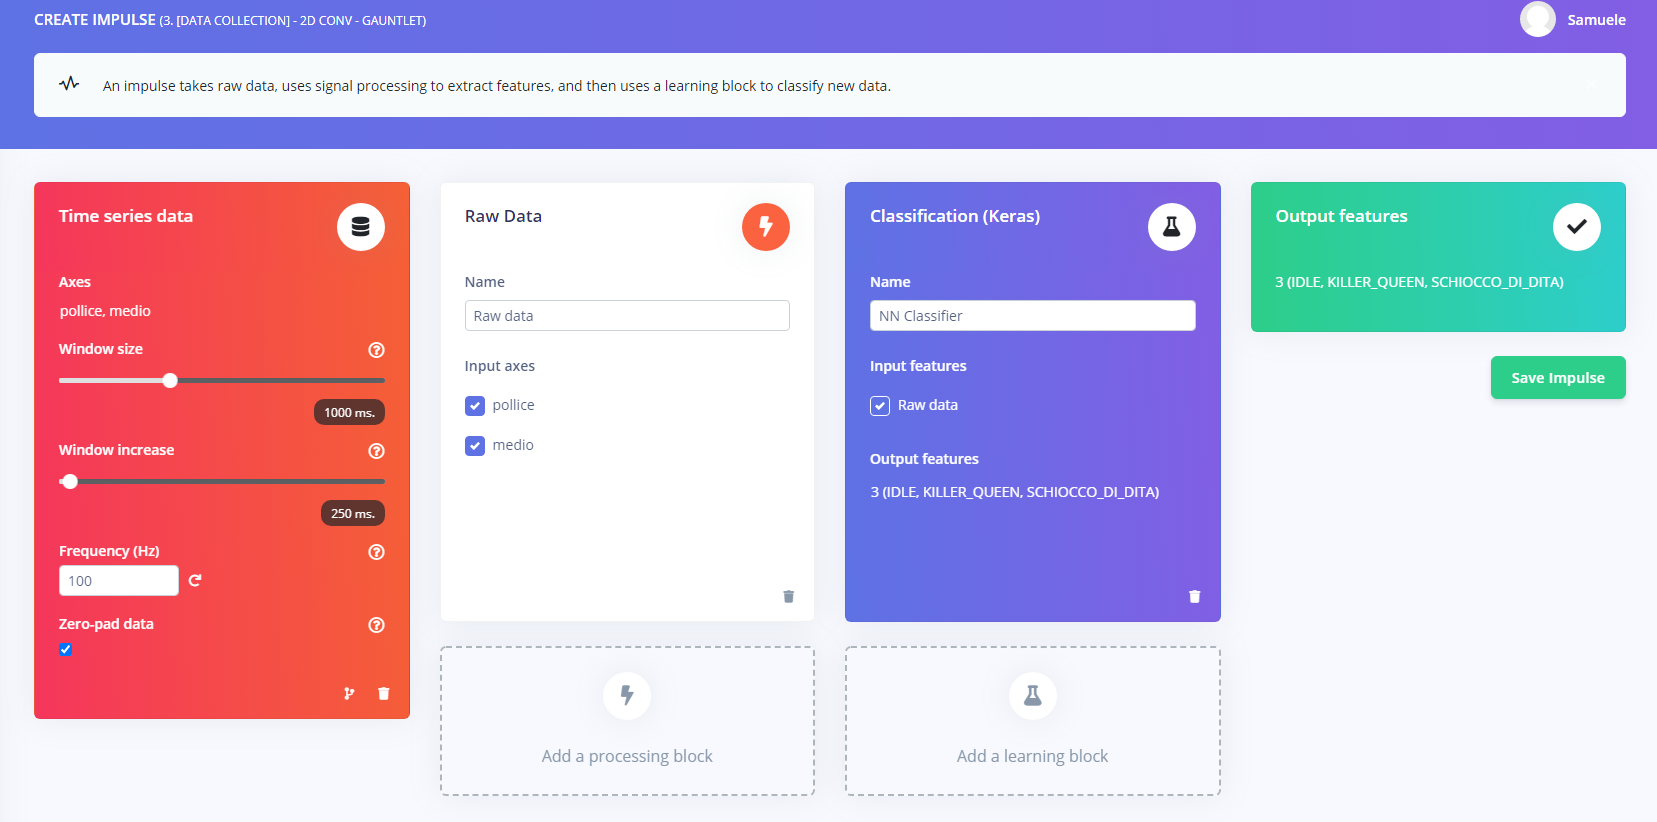
\includegraphics[width=\textwidth{}]{figures/Edge_Impulse_Impulso_Completo.PNG}
    \caption{Edge Impulse - Impulso Completo}
\end{figure}

\par{}'Time Series Data', indica principalmente la grandezza del vettore in ingresso al modello, rispetto al tempo (da qui la necessità del timestamp nel \riferimento{sezione 2-1-1}{Protocollo Edge Impulse}).
\par{}Il 'Blocco di Processo': 'Raw Data', indica che i dati ricevuti non dovranno essere modificati prima di essere passati alla rete neurale.
\par{}Mentre il 'Blocco di Apprendimento': 'Classification (Keras)', è una rete neurale costruita in python attraverso la libreria "keras" offerta da "TenserFlow".
\par{}Le 'Output Features', come accennato poco sopra sono i label digitati\comment{inseriti} durante l'upload dei file.\\

\newpage{}

\par{}A questo punto per completare l'Impulso è necessario specificare lo schema della rete neurale che dovrà essere utilizzata nel modello, dopo vari tentativi per testare quale potesse essere essere il miglior approccio, sono arrivato al seguente diagramma:
\label{IMAGE - NN CLASSIFIER}
\begin{figure}[H]
    \centering
    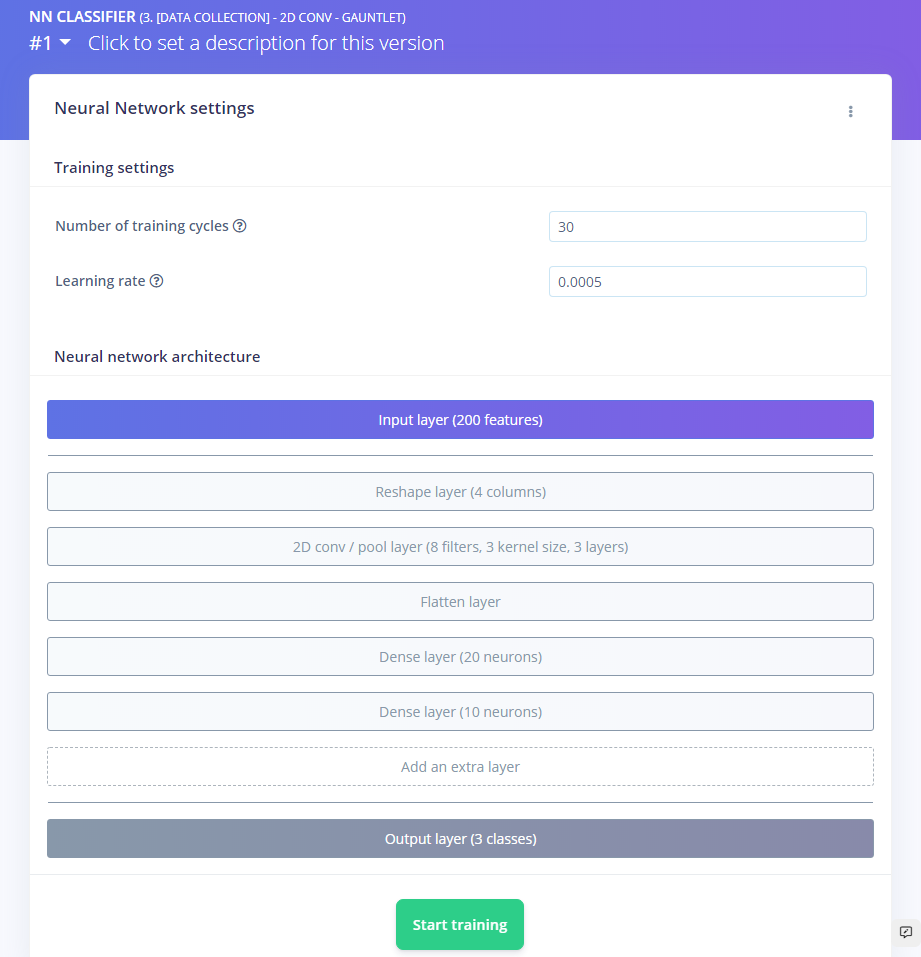
\includegraphics[width=\textwidth{}]{figures/Edge_Impulse_Gauntlet_NN_Classsifier.PNG}
    \caption{Edge Impulse - Rete Neurale}
\end{figure}

\newpage{}

Cliccando su "Start training", dopo pochi minuti, ci viene fornita oltre all'accuratezza rispetto al set di '\textit{cross-validation}', anche una stima delle prestazioni che avrà il modello una volta dislocato sulla piattaforma embedded scelta, ed una utile \textit{confusion matrix}, che indica per quale/i classi il modello ha una peggiore capacità di classificazione.
\label{IMAGE - TRAINING}
\begin{figure}[H]
    \centering
    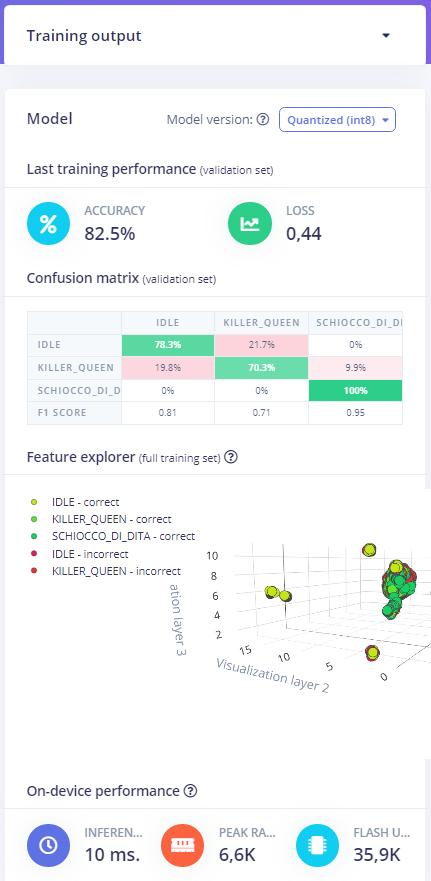
\includegraphics[width=90mm]{figures/Edge_Impulse_Training.PNG}
    \caption{Edge Impulse - Risultati Addestramento}
\end{figure}

La rete neurale è conclusa, rimane solo da portarla sulla scheda Arduino sotto forma di modello di TensorFlow Lite.\\
Rechiamoci quindi, alla parte di "\textit{Deployment}" di Edge Impulse e scegliamo l'opzione \\"\textit{Arduino Library}":
\label{IMAGE - DEPLOYMENT}
\begin{figure}[H]
    \centering
    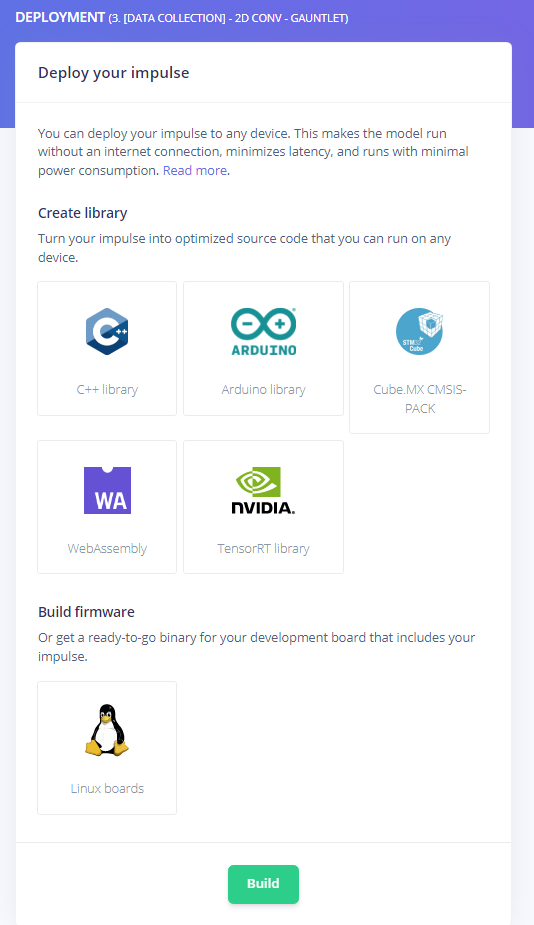
\includegraphics[width=100mm]{figures/Edge_Impulse_Deployment.PNG}
    \caption{Edge Impulse - Deployment}
\end{figure}
Ci verrà fornita una libreria ".zip" che potrà essere aggiunta dall'Arduino IDE da:\\ Sketch$\rightarrow{}$\#include libreria$\rightarrow{}$Aggiungi libreria da file .ZIP...




\section{Utilizzo della Libreria Offerta da Edge Impulse} \label{sezione 2-4}
Una volta scaricata la libreria da "Edge Impulse", la possiamo includere su un nuovo sketch Arduino, e caricare un codice esempio\comment{compreso nella} dalla stessa libreria, dal nome "static\_buffer":
\label{IMAGE - DEPLOYMENT}
\begin{figure}[H]
    \centering
    \caption{Arduino IDE - static\_buffer example}
    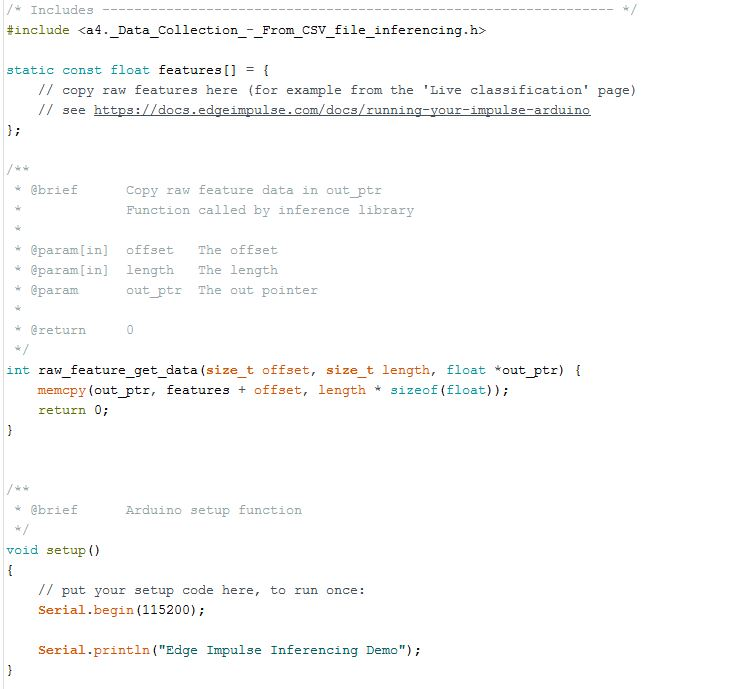
\includegraphics[width=\textwidth{}]{figures/Edge_static_buffer_Setup.JPG}
\end{figure}

\newpage{}

In questo esempio ci è consigliato di modificare, o meglio, riempire il vettore "features[ ]" con i dati presi dai sensori, quindi utilizzando lo stesso metodo per la raccolta dati, riempiamo il vettore:
\begin{lstlisting}[language=Arduino]
void loop(){
    int length_featrues = sizeof(features)/sizeof(float);
    for(int i = 1; i < length_features; i++){
        features[i-1] = features[i];
    }
    features[length_featrues-1] = new_data_just_aquired
}
\end{lstlisting}
Dopodiché nell'esempio il vettore viene passato in una serie di funzioni per poter poi essere usato dal classificatore, o rete neurale:
\begin{lstlisting}[language=Arduino]
    int raw_feature_get_data(size_t offset, size_t length, float *out_ptr) {
        memcpy(out_ptr, features + offset, length * sizeof(float));
        return 0;
    }

    // the features are stored into flash, and we don't want 
    // to load everything into RAM
    signal_t features_signal;
    features_signal.total_length = sizeof(features) / sizeof(features[0]);
    features_signal.get_data = &raw_feature_get_data;

    // invoke the impulse
    EI_IMPULSE_ERROR res = run_classifier(
    &features_signal, &result, false /* debug */);
    
    // -----------------------------------------------------------------------
    // TEMPI DEL CLASSIFICATORE
    // result.timing.dsp
    // result.timing.classification
    // result.timing.anomaly
    
    // DETTAGLI:
    // result.classification[ix].label
    // result.classification[ix].value
    // result.anomaly
\end{lstlisting}

Quindi con \lstinline{result.classification[ix].label}, \lstinline{result.classification[ix].value}, e \lstinline{result.anomaly} è possibile implementare il resto del codice:

\begin{lstlisting}[language=Arduino]
    if(result.classification[ix].label == "SCHIOCCO_DI_DITA"){
        if(result.classification[ix].value > 0.9){
            // Light the leds
            digitalWrite(A2, HIGH);
            
            // Empty features[] vector
            float new_blank_float[lenght_features];
            features = new_blank_float;
            
            delay(2000);
            
            // Kill the ligths
            digitalWrite(A2, LOW);
        }
    }
\end{lstlisting}

\myNOTE{
In questo caso \lstinline{result.anomaly} non è stata implementata. In caso si volesse implementare\\
è possibile, tornando alla costruzione dell'Impulso nella sezione precedente, aggiungendo\\
un nuovo "Blocco di Apprendimento" chiamato "Anomaly Detection (K-means)" che\\ 
tramite un algoritmo di K-clustering ritorna un valore, sempre tra 0 ed 1, indicativo di\\ 
quanto è probabile che la classificazione trovata sia un anomalia, in caso questo se il valore\\
fosse elevato, la classificazione va considerata errata e deve essere scartata.
}